\subsection{Active Target (ATAR)}
\begin{figure}[h!]
\centering
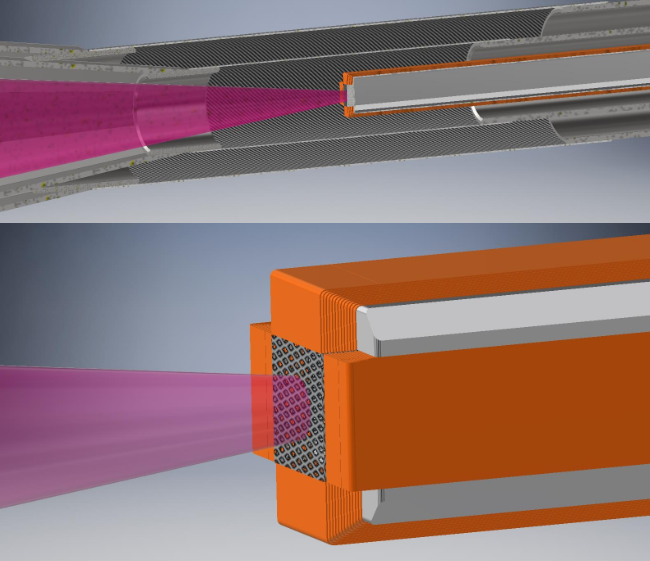
\includegraphics[scale=0.4]{sections/figures/atar1.png}
\caption{place holder: fig:atar1}
\label{fig:atar1}
\end{figure}

Fig.~\ref{fig:atar1} shows a concept drawing for  the pion beam entrance channel and  the active target. The  focused and collimated beam with a 1 cm diameter area passes through degrading plastic scintillators and two layers of double sided Si-strip detectors (not shown) before hitting the target. 
The stopping target (ATAR) is a rectangular prism of 20 mm transverse size and 5.76 mm in beam direction. It consists of 48 layers of AC LGAD sensors with a strip pitch of 200 $\mu m$. This results in 100 channels per layer and 4800 channels for the full detector. Consecutive layers are rotated by 90 degrees.

%Before describing the target (ATAR) in detail, let us recall its The target has the following functionalities:


\begin{itemize} 
\item 
Pion stops are identified. The expected stopping distributions are presented in fig.~\ref{fig:sim.stops}.
\begin{figure}[h!]
\centering

\includegraphics[scale=0.4]{sections/figures/ph.png}
\caption{place holder: fig:sim.stops}
\label{fig:sim.stops}
\end{figure}

\item
The $\pi \rightarrow \mu \rightarrow e$ Michel chain has to be suppressed by several orders of magnitude for measurement of the calorimeter energy response tail. The expected temporal pulse pair resolution of $dt\sim$1 ns provides a suppression factor of $\lambda_\pi dt=0.038$. An additional suppression results from a tight observation window of 
%several 
about one
pion lifetime, which disfavors the slower muon decay. Further separation is based on topology and energy 
deposition. Muons from pion decay have 4.1 MeV energy and a projected range of 0.8 mm in silicon. The $<$200 $\mu m$ segmentation of the detector was
chosen to resolve most tracks of isotropically emitted muons (see section~\ref{sec:simulation}). A zig-zag strip pattern will identify
the small fraction of muon tracks which stay within a layer and parallel to a strip. Fully depleted silicon detectors with minimal dead material
are essential to fully utilize the energy information. The required dynamic range of the readout is large as a pion can deposit 2 MeV in a
200 $\mu m$ range compared to 40 keV for a MIPS. \todo{MIPS number correct? Simone}

\item 
The "old" muons, accidental muons stops preceding the trigger signal, were a significant background in the previous generation of experiments by generating additional components in the time distributions
presented in fig.~\ref{fig:T1A}. In the PIENU experiment those were kept at an acceptable level, by imposing a wide pile-up window to -7 $\mu s$ before
the pion stop to let old muons decay, at the cost of 60\% of the statistics. For \nexp\, with its 
%5$\times$ 
higher beam rate, this is not 
%an option.
desirable.
Moreover the accidental rate will increase according to the increase of the beam rate. The much faster calorimeter will significantly reduce the pile-up contributions, which are more difficult to model and to determine correctly. In addition we will study how to reduce these accidentals by developing a local pileup rejection approach,
i.e. checking whether the observed decay electron belongs to the stopping vertex of the triggering pion.

\item
Muons arising from upstream pion decays are  relatively easily identified 
by their energy loss dE/dx properties and by  
kinks in their trajectories.
Pion decay
inside the target will be separated by kinks in the topology, dE/dx along the track, c.f. section~\ref{sec:simulation}, and range in the target. A sufficient Michel chain suppression and the tail suppression afforded by the 
%hermetic 
large acceptance
CALO will also allow  constraining a subtle background from Michel decays where the 4.1 MeV
 muon decays before leaving a track in the ATAR. 

\item
The ATAR will also be essential in defining event triggers. As will be discussed in section~\ref{section:daq}, the triggers will include
a relative simple CALO trigger based on all events above the Michel edge. An additional selective trigger based on fast ATAR tracking should suppress the $\pi-\mu-e$ sequence
to such extent, that the fully digitized ATAR information can be stored. The ultimate goal of this analysis is the offline suppression of Michel events so that the
low energy tail of the $\pi \rightarrow e \nu$ response can be measured in-situ. 

\end{itemize}



\todo{ATAR concept by Simone and Abe, please also sketch the readout. Need to address charge sharing. Peter sketched the ATAR readout in the DAQ section, as a starting point for Lawrence and Tim} 

While the LGAD ATAR design is the baseline option, we will also study a scintillating fiber option. Crossed planes of 250 $\mu m$ diameter
fibers should work well with the large signals expected. Recent developments in ultrafast fibers based on a new type of high performance nanostructured organosilicon luminophores (Kuraray NOL-11) and the  multi-channel  SiPM  array from  Hamamatsu  HPK  (S13552-HRQ) built for LHCb provide promising hardware components for this alternative.